\section{Introduction}\label{sec:intro}
The Large Hadron Collider (LHC) is created  to explore the fundamental  properties  of matter for the next decades. Since LHC start-up in 2009, the experiments has collected and distributed hundreds  of  petabytes  of  data worldwide to hundreds of computer centers. Thousands of physicists analyze petascale  data volumes daily. One of  the LHC experiments  the ATLAS  \cite{Aad:2008}  utilizes the PanDA  workload management system \cite{Maeno2011} (WMS) for distributed data processing and analysis. The ATLAS Computing model \cite{Atlas2005} is based on a Grid paradigm \cite{Foster:1998}, with multilevel, hierarchically distributed computing  and storage resources. Acronym  PanDa stands for Production  and Distributed Analysis, the system  has  been developed to meet growing ATLAS production and analysis requirements for a data-driven  workload  management system capable of operating at LHC data processing scale.
PanDA has a highly scalable architecture. Scalability  has been demonstrated in ATLAS through the rapid increase in usage over the past several years of operations, and is expected to meet the continuously growing number of jobs over the next decade. PanDA  was designed to have the flexibility to adapt to emerging computing  technologies in processing,  storage, networking  as well as the underlying software stack (middleware). This flexibility has also been successfully demonstrated through the past six years of evolving  technologies adapted by computing centers in ATLAS which span many continents and yet are seamlessly integrated into PanDA.
PanDA  manages a wide spectrum of workloads, ranging from raw data processing to Monte Carlo simulation and user analysis, while actively evolving to meet rapidly changing science needs.  Today, it  serves several  thousand users, successfully managing job distribution to hundreds of ATLAS sites with more than 100,000 CPU cores  which process  more than a million jobs per day, Figure 1 shows  a  summary   of daily completed jobs on ATLAS Grid for the past 12 month.
\begin{figure}
\begin{center}
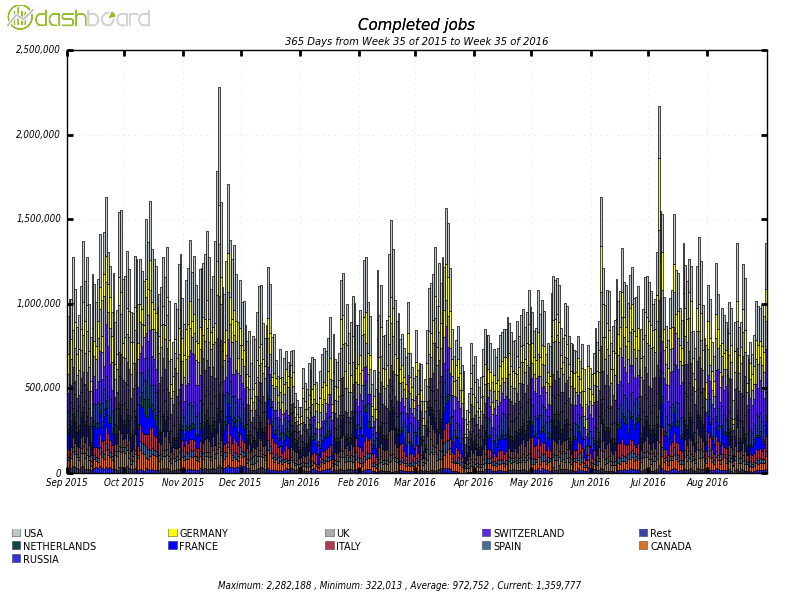
\includegraphics[width=\columnwidth]{figures/DailyJobs.png}
\caption{Daily completed jobs on ATLAS Grid\label{fig:daily}}
\end{center}
\end{figure}


